\documentclass[a4paper,12pt,dutch]{article}
\usepackage{glossaries}
\usepackage[T1]{fontenc}
\usepackage{babel}
\usepackage{graphicx}
\usepackage[table,xcdraw]{xcolor}
\usepackage{hyperref}
\usepackage{blindtext}
\usepackage{geometry}
\usepackage{parskip}
\usepackage{mathtools}
\usepackage{siunitx}
\usepackage{listings}
\usepackage{csquotes}

% %% Some packages you will need
% \usepackage{pgfplots}
% \usepackage{pgfplotstable}
% \usepackage{booktabs}
% \usepackage{array}
% \usepackage{colortbl}


\definecolor{arduinoorange}{HTML}{FFA500}
\definecolor{arduinogray}{HTML}{808080}
\definecolor{arduinoblue}{HTML}{007ACC}
\definecolor{arduinogreen}{HTML}{469B00}

\lstset{
  language=C++,
  basicstyle=\ttfamily\footnotesize,
  keywordstyle=\color{arduinoorange},
  stringstyle=\color{arduinogreen},
  commentstyle=\color{arduinogray},
  moredelim=[s][\color{arduinoblue}]{\#}{\ },
  morekeywords={digitalRead,digitalWrite,pinMode,analogRead,analogWrite,Serial,begin,HIGH,LOW},
  frame=tb,
  tabsize=4,
  showstringspaces=false,
  breaklines=true,
  numbers=left,
  numberstyle=\tiny\color{arduinogray},
  numbersep=5pt,
  extendedchars=true,
  literate={á}{{\'a}}1 {ã}{{\~a}}1 {é}{{\'e}}1,
}

\lstdefinestyle{Arduino}
{
  language=C++,
  basicstyle=\ttfamily\footnotesize,
  keywordstyle=\color{arduinoorange},
  stringstyle=\color{arduinogreen},
  commentstyle=\color{arduinogray},
  moredelim=[s][\color{arduinoblue}]{\#}{\ },
  morekeywords={digitalRead,digitalWrite,pinMode,analogRead,analogWrite,Serial,begin},
  frame=tb,
  tabsize=4,
  showstringspaces=false,
  breaklines=true,
  numbers=left,
  numberstyle=\tiny\color{arduinogray},
  numbersep=5pt,
  extendedchars=true,
  literate={á}{{\'a}}1 {ã}{{\~a}}1 {é}{{\'e}}1,
  backgroundcolor=\color{black!85},
  rulecolor=\color{arduinoorange},
  frame=single,
  frameround=tttt,
  framexleftmargin=6pt,
  framexrightmargin=6pt,
  framextopmargin=6pt,
  framexbottommargin=6pt,
  breaklines=true,
  postbreak=\raisebox{0ex}[0ex][0ex]{\ensuremath{\color{red}\hookrightarrow\space}},
}


\usepackage[
    backend=biber,
    backref=true,
    backrefstyle=none,
    sortcites=true,
    sorting=none,
    doi=false, % doi informatie wordt niet weergegeven
    %uniquename=true,
    %uniquelist=true,
    maxcitenames=3,
    %issn=false, werkt niet
    language=american
]{biblatex}
\addbibresource{Bronnen.bib}
\DefineBibliographyStrings{dutch}{
    backrefpage = {blz.},
    backrefpages = {blz.},
}
\makeglossaries
\definecolor{Grey1}{HTML}{343434}
\graphicspath{{./Media/Figuren/}}
 \geometry{
 a4paper,
 total={170mm,257mm},
 left=20mm,
 top=20mm,
 }
\hypersetup{
    colorlinks=true,
    linkcolor=blue,
    filecolor=magenta,      
    urlcolor=cyan,
    pdftitle={Overleaf Example},
    pdfpagemode=FullScreen,
    }

\begin{document}
\title{

\includegraphics[width=3.5in]{Media/Figuren/HHS.png} \\
\vspace*{2in}
\textbf{Ingenieursvaardigheden 3}\\
\textit{Studieloopbaan begeleiding}\\
Versie 1.0
}
\author{
\vspace*{1.5in} \\
  Geschreven door:\\
  Laurens van der Drift\\
		\vspace*{1in} \\
		De Haagse Hogeschool\\
        \textbf{Elektrotechniek}\\
        Delft, Nederland
       } 
\maketitle
% \section{Verklarende Woordenlijst}
%\addcontentsline{toc}{section}{Verklarende Woordenlijst}
\printglossaries

\newglossaryentry{ect.}{
  name = {ect.},
  description = {De betekenis van de Latijnse combinatie et cetera is 'enzovoort'. Voor et cetera wordt de afkorting etc.}
}

\newglossaryentry{DC}{
  name = {DC},
  description = {Direct Current (DC) is een elektrische stroom die in één richting vloeit, in tegenstelling tot wisselstroom (AC) waarin de stroomrichting periodiek omkeert.}
}

\newglossaryentry{gelijkstroomdistributiesysteem}{
  name = {gelijkstroomdistributiesysteem},
  description = {Een gelijkstroomdistributiesysteem verwijst naar een elektrisch distributiesysteem dat gebruikmaakt van gelijkstroom (DC) in plaats van wisselstroom (AC) om elektrische energie te transporteren en te verdelen.}
}

\newglossaryentry{DC-microgrids}{
  name = {DC-microgrids},
  description = {DC-microgrids zijn kleine, zelfvoorzienende elektrische netwerken die gelijkstroom (DC) gebruiken om energie lokaal op te wekken, op te slaan en te distribueren, vaak voor specifieke toepassingen of gebieden.}
}

\newglossaryentry{DC-netwerken}{
  name = {DC-netwerken},
  description = {DC-netwerken verwijzen naar elektrische netwerken die gebaseerd zijn op gelijkstroom (DC) in plaats van wisselstroom (AC) om elektriciteit te transporteren en te verdelen.}
}

\newpage
\tableofcontents
% % \section{Inleiding}
% Als onderdeel van het realiseren van een engineeringontwerp heb ik een volledige en correcte implementatie van het programma van eisen ontworpen. Het ontwerp dat ik heb gemaakt omvat een \gls{Smart-Car} dat gebruikmaakt van verscheidene sensoren om objecten te detecteren, een motorshield om de beweging van het apparaat te regelen, en een underglow LED-strip om het apparaat zichtbaarder te maken.

% \section{Bijeenkomsten}
De afgelopen periode heb ik deelgenomen aan vijf bijeenkomsten georganiseerd door \gls{YER}, die gericht waren op effectieve communicatie en samenwerking. Gedurende deze bijeenkomsten hebben we onze kennis op dit gebied vergroot. Wat mij het meest is bijgebleven, is de benadering van communicatie aan de hand van \gls{DISC}-profielen.

Nu ik beter begrijp hoe mijn team functioneert en hoe ze in verschillende situaties reageren, kan ik een nauwkeuriger profiel van elk teamlid samenstellen en ze beter aansturen. Als projectleider kan ik hiermee conflicten voorkomen en ervoor zorgen dat de juiste mensen samenwerken aan de juiste taken. Door dit te doen, werkt mijn team gezamenlijk aan het oplossen van problemen en worden kennis en ervaring gecombineerd. Dit versterkt de onderlinge band binnen het team.

Tijdens de bijeenkomsten ben ik tot nieuwe inzichten gekomen, die ik nu onbewust toepas. Zo is mij bijvoorbeeld geleerd om geduldiger te zijn en meer tijd te nemen voor mijn team, zodat ze in alle rust kunnen werken. Echter, zodra we van het tijdschema afwijken, neem ik de leiding en stuur ik iedereen adequaat aan om ervoor te zorgen dat de benodigde resultaten op-tijd worden behaald. Ik ben me er ook van bewust dat het soms noodzakelijk is om tijdelijk te stoppen met het uitvoeren van een bepaalde taak, als dit de beste strategie blijkt te zijn.

Kortom, deze bijeenkomsten hebben mij waardevolle inzichten verschaft over effectieve communicatie en samenwerking. Ik ben in staat gebleken deze inzichten toe te passen, waarbij ik mijn team beter kan aansturen en conflicten kan voorkomen. Tevens heb ik geleerd om flexibel te zijn en situaties op de juiste manier te benaderen, wat resulteert in een efficiëntere en succesvollere samenwerking met mijn teamleden.

% \section{Motorshield}
% Om het motorshield aan te sturen, heb ik onderzocht welke componenten zich op het shield bevonden en hoe ik deze kon aansturen. Ik heb de schematische tekening (figuur \ref{MSCHEM}) bekeken en gezien welke poorten aan welke motoren waren verbonden.
% \begin{figure}[h]
%     \centering
%     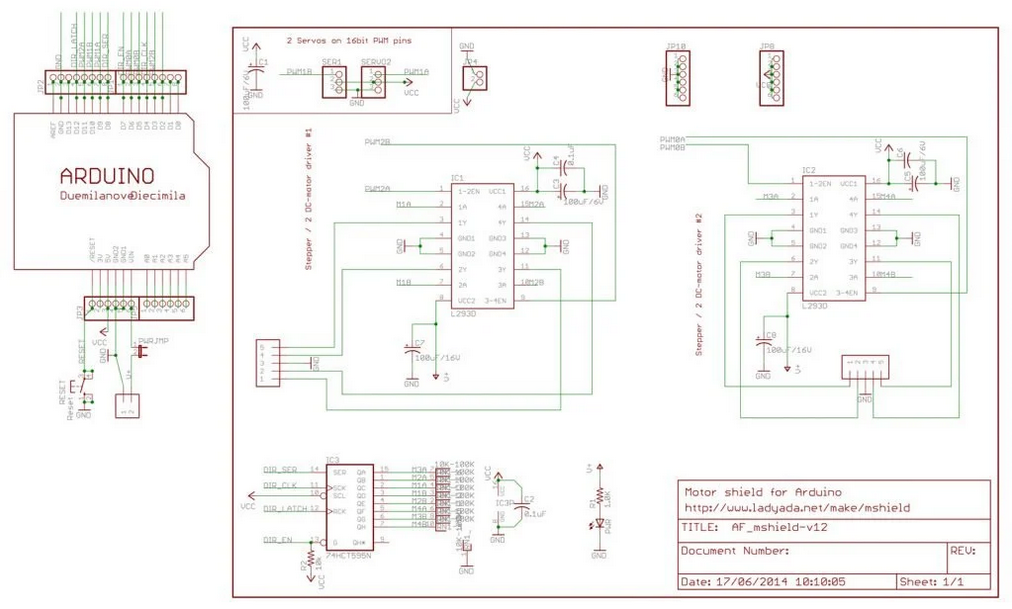
\includegraphics[scale=.3]{Media/Figuren/Motorshield_SCHEM.png}
%     \caption{Motorshield schematische tekening}
%     \label{MSCHEM}
% \end{figure}


% Met behulp van de timingtabel in figuur \ref{Timing} heb ik code geschreven waarmee we de 8-bits code uit figuur \ref{MCode} kunnen sturen naar het motorshield.
% \begin{figure}[h]
%     \centering
%     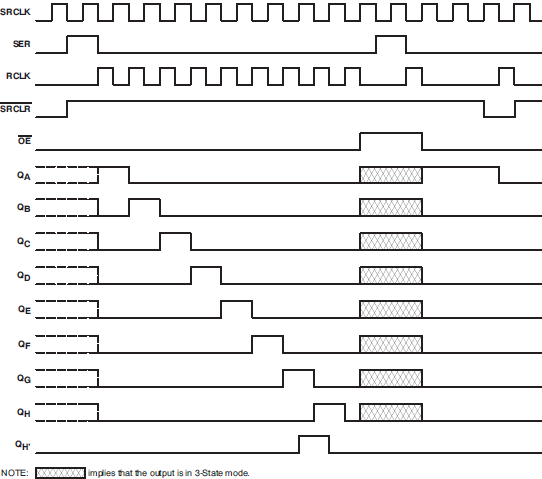
\includegraphics[scale=.5]{Media/Figuren/Timing.PNG}
%     \caption{Motorshield timing}
%     \label{Timing}
% \end{figure}

% \begin{figure}[h]
%     \begin{lstlisting}
%     void MOTOR(int Direction, int MotorPWM1, int MotorPWM2, int MotorPWM3, int MotorPWM4) {
%   SPEED(MotorPWM1, MotorPWM2, MotorPWM3, MotorPWM4);
%   digitalWrite(DIR_LATCH, LOW);
%   shiftOut(DATA, DIR_CLK, MSBFIRST, Direction);
%   digitalWrite(DIR_LATCH, HIGH);}
%     \end{lstlisting}
%     \caption{Motorshield code}
%     \label{MCode}
% \end{figure}

% Met behulp van deze informatie heb ik een Excel-script geschreven waarmee we konden aangeven welke motor moest draaien en in welke richting. Deze gegevens hebben we later naar het shiftregister gestuurd, dat de H-brug aanstuurt.
% \section{Het eerste jaar van de opleiding}
\subsection{Competenties}
\subsubsection{Analyseren}
Voor onze \gls{Smart-Car} heb ik een model gecreëerd in de vorm van een \gls{flowchart}, waardoor we de \gls{Smart-Car} beter konden analyseren en de gemaakte keuzes konden begrijpen. Hoewel we de \gls{Smart-Car} zelf hebben geprogrammeerd, waren er momenten waarop we de keuzes van de \gls{Smart-Car} niet helemaal begrepen. Dankzij deze \gls{flowchart} konden we de regels en functionaliteiten beter analyseren. De \gls{flowchart} bood ons veel overzicht en structuur.
\subsubsection{Ontwerpen}
Afgelopen periode heb ik uitstekend gepresteerd. Dit heb ik bereikt door een negen-assige sensor toe te voegen, \gls{underglow} te installeren en een radiofrequente controller te ontwikkelen. Ik heb hier veel tijd in geïnvesteerd, maar uiteindelijk ben ik tot de conclusie gekomen dat het voor mij niet meer haalbaar is om de radiofrequente controller te maken vanwege tijdgebrek en defecte aangeleverde componenten.
\subsubsection{Realiseren}
Afgelopen periode heb ik hard gewerkt aan het herassembleren van de auto om ervoor te zorgen dat deze steviger en beter wordt. Hierdoor zullen er minder componenten los trillen. Daarnaast hebben we ons proces gefilmd en de video gepubliceerd op het Instagram-account van de Haagse Hogeschool. Bovendien heb ik veel tijd besteed aan het voortdurend optimaliseren van de code om ervoor te zorgen dat alles optimaal draait.

\href{https://www.instagram.com/reel/CpfstIiKLpz/?utm_source=ig_web_copy_link&igshid=MzRlODBiNWFlZA==}{Video 1},
\href{https://www.instagram.com/reel/CqDmm-vK4Lq/?utm_source=ig_web_copy_link&igshid=MzRlODBiNWFlZA==}{Video 2},
\href{https://www.instagram.com/reel/CqqS0jyOCNk/?utm_source=ig_web_copy_link&igshid=MzRlODBiNWFlZA==}{Video 3},
\href{https://www.instagram.com/reel/CrI-imUqiAH/?utm_source=ig_web_copy_link&igshid=MzRlODBiNWFlZA==}{Video 4}
\subsubsection{Professionaliseren}
Zoals besproken onder het kopje "Realiseren", was ik onder andere verantwoordelijk voor het behalen van excelleer opgaves. Mijn teamgenoten waren bezig met het realiseren van de radiofrequente controller. Op een gegeven moment heb ik besloten om de stekker eruit te trekken. Het behalen van uitstekende resultaten kostte te veel tijd en moeite. Dit resulteerde in te veel tijd die we eraan besteedden, waardoor we in tijdnood kwamen om aan de beoordelingsdoelen te voldoen. Bovendien heb ik bij opgelopen vertraging zonder duidelijke reden adequaat gereageerd op de situatie.
\subsection{Het eerste jaar}
Het eerste jaar van mijn opleiding is een zeer positieve ervaring geweest. Ik voel me erg op mijn plek en geniet van mijn omgeving, medestudenten, docenten en de elektronica. Het geeft me veel voldoening om me echt thuis te voelen. Daarnaast heb ik nu een leuke groep medestudenten met wie ik buiten school veel plezier beleef, zoals samen sporten of iets eten. Ik heb persoonlijk mijn doelen behaald. Ik heb ontzettend veel geleerd tijdens de opleiding en mijn kennis enorm verbreed. Ondanks dat er altijd tegen me is gezegd dat ik beter een studie zonder wiskunde kon kiezen, ben ik erg trots op mezelf.

Het meest waardevolle wat ik heb geleerd, is dat ik nu een groep mensen om me heen heb waarbij ik echt mezelf kan zijn, zonder dat ik meteen als een "nerd" word gezien. Op professioneel gebied heb ik geleerd hoe ik met verschillende situaties en teamprojecten moet omgaan. Ik kan nu beter intern communiceren en inschatten wat wel en niet haalbaar is.

Wat mij nog steeds interesseert, is hoe ik mijn structuur nog efficiënter kan maken, zodat ik minder tijd nodig heb om dingen af te krijgen en de lesstof beter te begrijpen.
% \include{Chapters/Underglow}
% % \section{Samenvatting}
% \subsection{Controller}
% In dit project is een op afstand bestuurbare auto ontwikkeld met behulp van een controller en een Bluetooth-module. De controller bestaat uit verschillende componenten, waaronder een TFT-display met een ili9341 IC, twee KY-023 joysticks en een krachtige microcontroller genaamd ESP32 D1 MINI, die draadloze verbindingen kan maken en complexe taken kan uitvoeren. Na het uitlezen van de waarden van de joysticks worden deze gekalibreerd en omgezet in een serieel formaat dat verzonden kan worden via de RF433MHZ-transceiver. De combinatie van RF433MHZ en de joysticks zorgt voor een betrouwbare en responsieve verbinding tussen de controller en de auto, waardoor de auto met precisie in elke richting kan worden bestuurd.

% \subsection{Motoraansturing}
% Om de vier motoren van de zelfrijdende auto aan te sturen, wordt gebruik gemaakt van een motorshield dat bestaat uit een 74HC595N shift-register en twee L293D H-brug motor drivers. Het shift-register creëert 8-bits extra digitale uitgangen zonder extra pinnen op de microcontroller te gebruiken en wordt gebruikt om gegevens naar de chip te sturen. De uitgangslatches van het shift-register sturen een positief of negatief signaal naar de L293D H-brug motor drivers, waarmee de motoren worden aangestuurd. Om een DC-motor in één richting te laten draaien, moeten de logische waarden op IN1 en IN2 voor motor 1 respectievelijk op HIGH en LOW worden gezet. De maximale PWM-waarde voor de motoren mag niet hoger zijn dan 220 om doorbranden van de motoren te voorkomen. Het is belangrijk om de stroomsterkte van de motor en het voltage van de voeding goed te controleren en af te stemmen op de specificaties van de L293D, die een maximale stroom van 600 mA per kanaal kan leveren en is uitgerust met ingebouwde beveiligingsfuncties, zoals thermische beveiliging uitschakeling en bescherming tegen kortsluiting, wat het veilig en betrouwbaar maakt om te gebruiken in diverse toepassingen.

% \subsection{Sensoren}
% Voor de zelfrijdende auto zijn sensoren gebruikt om objecten te detecteren en afstanden en oriëntatie te meten. Er zijn infrarood sensoren gebruikt voor het detecteren van objecten van 2 tot 30 centimeter en ultrasone sensoren voor het meten van afstanden tot 4 meter. Daarnaast is er een 9-assige oriëntatiesensor, genaamd de BNO055, die wordt gebruikt om de oriëntatie van de auto in de ruimte te meten. Voor de eisen van het project zijn er vier extra infrarood sensoren geplaatst, zodat de auto makkelijker door zijn omgeving kan manoeuvreren. De infrarood sensoren en de ultrasone sensoren zijn gepositioneerd aan de voorkant, achterkant en zijkanten van de auto. De sensoren kunnen worden aangestuurd via een protocol waarbij verschillende configuratieparameters kunnen worden ingesteld.
\section{Gastspreker 1}
Bij deze spreker was ik niet aanwezig dus kan ik geen antwoord geven op devolgende vragen:
\begin{itemize}
    \item Achtergrondinformatie van de gastspreker: naam, leeftijd, vakgebied, functie, organisatie, ect.
    \item Wat maakte je nieuwsgierig in zijn/haar verhaal?
    \item Welke competenties herken je in het verhaal van de gastspreker?
    \item Ga na welke kennis, vaardigheden en houding je moet hebben om deze competenties goed uit te kunnen voeren.
    \item Welke vraag/vragen heb je de gastspreker gesteld en wat was het antwoord?
    \item Wat is je het meest bijgebleven?
\end{itemize}
\subsection{Wie is Laurens?}
Laurens MacKay van DC Opportunities lijkt een expert te zijn op het gebied van gelijkstroom (direct current, DC) microgrids en DC-distributienetwerken. Hij heeft een grote academische achtergrond in elektrische techniek en informatietechnologie en heeft zowel een bachelor als een mastergraad behaald aan ETH Zurich in Zwitserland. Tijdens zijn master's thesis begon hij in 2012 te werken aan DC-distributienetwerken. Later, aan de Technische Universiteit Delft in Nederland, behaalde hij zijn doctoraat in 2018, waarbij zijn proefschrift betrekking had op "Stappen naar het universele gelijkstroomdistributiesysteem" (Steps Towards the Universal Direct Current Distribution System).\cite{LaurensLINKEDIN}
\subsection{Wie is DC Opportunities?}
Het bedrijf DC Opportunities, opgericht door Dr. Laurens Mackay, richt zich op de ontwikkeling van technologieën en toepassingen voor DC-microgrids en DC-distributienetwerken. Een specifiek project waarbij DC Opportunities betrokken is, heet "The Green Village," waarin ze samenwerken met CityTec om prototypes te ontwikkelen en testen voor het opladen van elektrische voertuigen (EV's) met behulp van bestaande DC-netwerken of kabels die zijn aangelegd voor straatverlichting op DC. Het doel is om elektrisch opladen in de toekomst gemakkelijker en kostenefficiënter te maken. \cite{DCSITE} \cite{DCLINKEDIN} \cite{Innovation_Quarter}
\subsection{Samengevat}
Kortom, Laurens MacKay en DC Opportunities richten zich op de bevordering van DC-technologieën en het verbeteren van DC-microgrids en distributienetwerken, met als doel het efficiënter maken van elektrische systemen en het ondersteunen van groene energie-initiatieven zoals elektrisch vervoer.
\phantomsection
\addcontentsline{toc}{section}{Referenties}
\printbibliography
% \phantomsection
\addcontentsline{toc}{section}{Metingen stroomverbruik}
% Please add the following required packages to your document preamble:
% \usepackage[table,xcdraw]{xcolor}
% If you use beamer only pass "xcolor=table" option, i.e. \documentclass[xcolor=table]{beamer}
\begin{table}[]
\begin{tabular}{ll}
\rowcolor[HTML]{4472C4} 
\multicolumn{1}{c}{\cellcolor[HTML]{4472C4}{\color[HTML]{FFFFFF} \textbf{Spanning (V)}}} &
  \multicolumn{1}{c}{\cellcolor[HTML]{4472C4}{\color[HTML]{FFFFFF} \textbf{\begin{tabular}[c]{@{}c@{}}Stroom\\ (A)\end{tabular}}}} \\
\rowcolor[HTML]{FFFFFF} 
\textit{\textbf{1}} & 0.253 \\
\rowcolor[HTML]{D9E1F2} 
2                   & 0.314 \\
\rowcolor[HTML]{FFFFFF} 
3                   & 0.362 \\
\rowcolor[HTML]{D9E1F2} 
4                   & 0.410 \\
\rowcolor[HTML]{FFFFFF} 
5                   & 0.454 \\
\rowcolor[HTML]{D9E1F2} 
\textit{\textbf{6}} & 0.459 \\
\rowcolor[HTML]{FFFFFF} 
7                   & 0.527 \\
\rowcolor[HTML]{D9E1F2} 
8                   & 0.564 \\
\rowcolor[HTML]{FFFFFF} 
9                   & 0.606 \\
\rowcolor[HTML]{D9E1F2} 
10                  & 0.649 \\
\rowcolor[HTML]{FFFFFF} 
11                  & 0.691 \\
\rowcolor[HTML]{D9E1F2} 
12                  & 0.747
\end{tabular}
\end{table}



% \pgfplotstableset{% global config, for example in the preamble
%   every head row/.style={before row=\toprule,after row=\midrule},
%   every last row/.style={after row=\bottomrule},
%   fixed,precision=2,
% }






% \pgfplotstabletypeset[
%   columns/Spanning/.style={column name=Spanning},
%   columns/Stroom/.style={column name=Stroom},
% ]{/table.txt}

% \begin{figure}[h!]
% \centering
% \begin{tikzpicture}
% \begin{axis}[
%     xlabel={Spanning},
%     ylabel=Stroom,
%     legend pos=south east,
%     legend entries={Concrete,Linoleum},
%     ]
%   \addplot table [x=freq,y=Spanning] {/table.txt};
%   \addplot table [x=freq,y=Stroom] {/table.txt};
% \end{axis}
% \end{tikzpicture}
% \end{figure}
\end{document}